From equations (4.22) one might be tempted to try to implement SOR as
\begin{verbatim}
     for iter=1:maxiter
        uGS = (DA - LA) \ (UA*u + rhs);
        u = u + omega * (uGS - u);
     end
\end{verbatim}

where the matrices have been defined as in \verb+iter_bvp_Asplit.m+. Try this computationally and observe that it does
not work well. Explain what is wrong with this and derive the correct expression (4.24).

\begin{solution}\ \\\\
    We implement the above SOR algorithm as the \texttt{naive\_SOR} case in \texttt{problem\_1d.m}. The corresponding
    error plot is shown below:

    \begin{figure}[h]
        \centering
        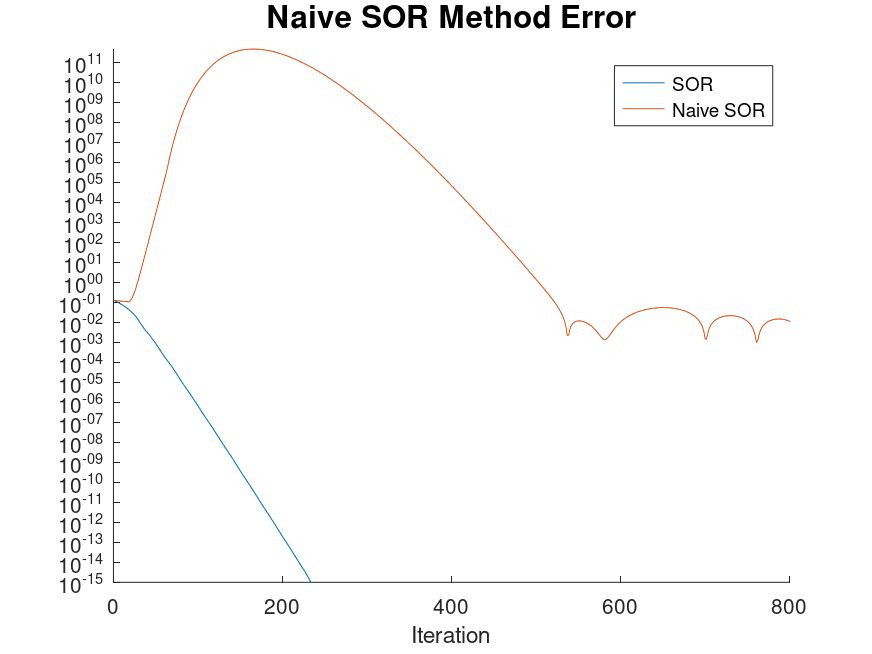
\includegraphics[width=0.7\textwidth]{problem_1d_naive_sor_matrix_splitting_error_800_iterations.png}
        \caption{Comparison of Naive SOR implementation and Correct SOR implementation}
    \end{figure}

    The above naive two-step formulation amplifies the error in each GS step by a factor of $\omega$ before applying
    the iteration update. (I \textbf{think} this is what's wrong with this method).

    To derive (4.24), we first recall the Gauss-Seidel update:

    \begin{equation}
        u_i^{GS} = \frac{1}{2} \left( u_{i-1}^{[k+1]} + u_{i+1}^{[k]} - h^2 f_i \right) \\
    \end{equation}

    \pagebreak
    We substitute (1) into our SOR update step to find:

    \begin{align*}
        u_i^{k+1} &= u_i^{[k]} + \omega \left( u_i^{GS} - u_i^{[k]} \right) \\
                  &= u_i^{[k]} + \omega \left[ \frac{1}{2} \left( u_{i-1}^{[k+1]} + u_{i+1}^{[k]} - h^2 f_i \right) - u_i^{[k]} \right] \\
                  &= (1 - \omega) u_i^{[k]} + \frac{\omega}{2} \left( u_{i-1}^{[k+1]} + u_{i+1}^{[k]} - h^2 f_i \right). \\
    \end{align*}

    We collect all $[k+1]$ iteration terms on the left and all other terms on the right to find:

    \begin{equation}
        2 u_i^{k+1} - \omega u_{i-1}^{[k+1]} = 2 (1 - \omega) u_i^{[k]} + \omega u_{i+1}^{[k]} - \omega h^2 f_i \\
    \end{equation}

    If we recall that $D$ and $L$, and $U$ are given by

    \[
    D = -\frac{1}{h^2} \begin{pmatrix} 
         2 &       0 \\
         0 &       2 &      0 \\
           & \ddots & \ddots & \ddots \\
           &        &      0 &      2 &  0 \\
           &        &        &      0 &  2 
    \end{pmatrix},\;
    L = -\frac{1}{h^2} \begin{pmatrix} 
         0 &       0 \\
         1 &       0 &      0 \\
           & \ddots & \ddots & \ddots \\
           &        &      1 &      0 & 0 \\
           &        &        &      1 & 0 
    \end{pmatrix}, \;
    U = L^T
    \]

    then (2) becomes:

    $$
        (D - \omega L) \textbf{u}^{[k+1]} = \left[(1 - \omega) D + \omega U \right] \textbf{u}^{[k]} + \omega f_i
    $$

    Lastly, we divide by $\omega$ which yields:

    $$
        \frac{1}{\omega} (D - \omega L) \textbf{u}^{[k+1]} = \frac{1}{\omega} \left[(1 - \omega) D + \omega U \right] \textbf{u}^{[k]} + f_i
    $$

    and hence 

    \begin{align*}
        M &= \frac{1}{\omega} (D - \omega L) \\
        N &= \frac{1}{\omega} \left[(1 - \omega) D + \omega U \right]
    \end{align*}

    as desired.
    \ \\
\end{solution}